%
% Credit to Tibault Reveyrand for the initial template - https://www.overleaf.com/articles/ieee-journal-submission-trans-on-mtt-example/pbfcbcjvmvmn

% ================================================
% Please HIGHLIGHT the new inputs such like this :
% Text :
%  \hl{comment}
% Aligned Eq. 
% \begin{shaded}
% \end{shaded}
% ================================================


\documentclass[journal]{IEEEtran}

%\usepackage[retainorgcmds]{IEEEtrantools}
%\usepackage{bibentry}  
\usepackage{xcolor,soul,framed} %,caption

\colorlet{shadecolor}{yellow}
% \usepackage{color,soul}
\usepackage[pdftex]{graphicx}
\graphicspath{{../pdf/}{../jpeg/}}
\DeclareGraphicsExtensions{.pdf,.jpeg,.png}

\usepackage[cmex10]{amsmath}
%Mathabx do not work on ScribTex => Removed
%\usepackage{mathabx}
\usepackage{array}
\usepackage{mdwmath}
\usepackage{mdwtab}
\usepackage{eqparbox}
\usepackage{url}

\hyphenation{op-tical net-works semi-conduc-tor}

%\bstctlcite{IEEE:BSTcontrol}


%=== TITLE & AUTHORS ====================================================================
\begin{document}
\bstctlcite{IEEEexample:BSTcontrol}
    \title{Screening  Radiology  Images  for Lesion  Detection: An ML Approach}
  \author{Teodor~Ilie,~Jihye    on~Park,~and~Alex~Sun% <-this % stops a space

}  

% The paper headers
\markboth{}{}

% ====================================================================
\maketitle


% === 1. ABSTRACT ====================================================================
% =================================================================================
\begin{abstract}
%\boldmath
This is the abstract.
\end{abstract}

\begin{IEEEkeywords}
Radiology, DeepLesion, Convolutional Neural Network, U-Net, YOLO
\end{IEEEkeywords}


% === II. BACKGROUND =============================================================
% =================================================================================
\section{Background}

% =======
% FIG. 01
% =======
% \begin{figure}
%  \begin{center}
%  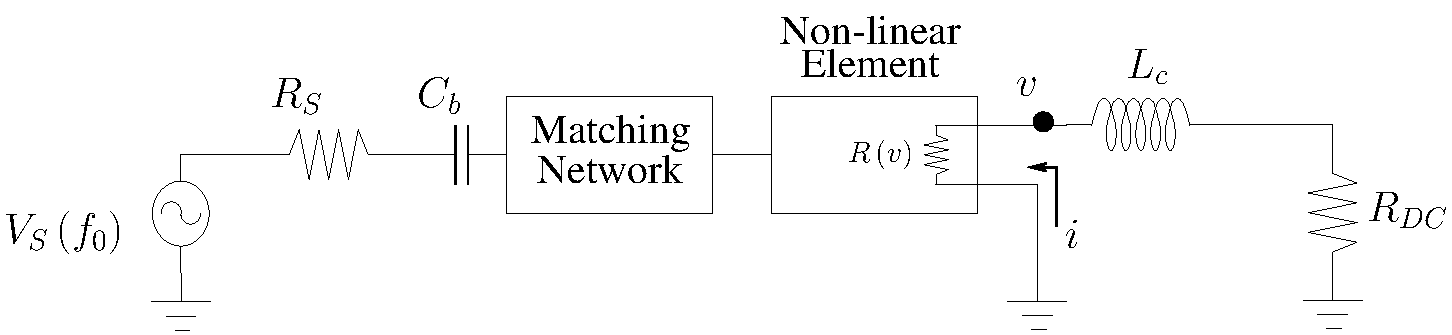
\includegraphics[width=3.5in]{pdf/01.pdf}\\
%  \caption{Caption}\label{circuit_diagram}
%  \end{center}
%\end{figure}

\IEEEPARstart{C}{omputed} Tomography (CT) scans produce dozens, even hundreds of images of cross-sectional slices of patients, which may contain tumorous lesions indicative of cancer. However, when a radiologist is searching through these images, they are not always looking for tumorous lesions. This is also an incredibly time-consuming process, and the lesions could often be missed by the radiologist. We propose an ML model which automatically analyzes individual CT scan slices, efficiently and accurately detecting and highlighting lesions in the images for closer inspection by a radiologist.  This would serve as an immensely useful tool to assist radiologists with making early cancer diagnoses, potentially saving lives.


% === III. HYPOTHESIS ========================
% =================================================================================
\section{Hypothesis}
Hypothesis\cite{deeplesion}

% === IV. METHODS ========================
% =================================================================================
\section{Methods}

% === V. RESULTS ========================
% =================================================================================
\section{Results}

% === VI. DISCUSSION ========================
% =================================================================================
\section{Discussion}


\section*{Team Reflection}

\bibliographystyle{IEEEtran}
\bibliography{IEEEabrv,Bibliography}

\vfill
\end{document}

% An example of a floating figure using the graphicx package.
% Note that \label must occur AFTER (or within) \caption.
% For figures, \caption should occur after the \includegraphics.
% Note that IEEEtran v1.7 and later has special internal code that
% is designed to preserve the operation of \label within \caption
% even when the captionsoff option is in effect. However, because
% of issues like this, it may be the safest practice to put all your
% \label just after \caption rather than within \caption{}.
%
% Reminder: the "draftcls" or "draftclsnofoot", not "draft", class
% option should be used if it is desired that the figures are to be
% displayed while in draft mode.
%
%\begin{figure}[!t]
%\centering
%\includegraphics[width=2.5in]{myfigure}
% where an .eps filename suffix will be assumed under latex, 
% and a .pdf suffix will be assumed for pdflatex; or what has been declared
% via \DeclareGraphicsExtensions.
%\caption{Simulation Results}
%\label{fig_sim}
%\end{figure}

% Note that IEEE typically puts floats only at the top, even when this
% results in a large percentage of a column being occupied by floats.


% An example of a double column floating figure using two subfigures.
% (The subfig.sty package must be loaded for this to work.)
% The subfigure \label commands are set within each subfloat command, the
% \label for the overall figure must come after \caption.
% \hfil must be used as a separator to get equal spacing.
% The subfigure.sty package works much the same way, except \subfigure is
% used instead of \subfloat.
%
%\begin{figure*}[!t]
%\centerline{\subfloat[Case I]\includegraphics[width=2.5in]{subfigcase1}%
%\label{fig_first_case}}
%\hfil
%\subfloat[Case II]{\includegraphics[width=2.5in]{subfigcase2}%
%\label{fig_second_case}}}
%\caption{Simulation results}
%\label{fig_sim}
%\end{figure*}
%
% Note that often IEEE papers with subfigures do not employ subfigure
% captions (using the optional argument to \subfloat), but instead will
% reference/describe all of them (a), (b), etc., within the main caption.


% An example of a floating table. Note that, for IEEE style tables, the 
% \caption command should come BEFORE the table. Table text will default to
% \footnotesize as IEEE normally uses this smaller font for tables.
% The \label must come after \caption as always.
%
%\begin{table}[!t]
%% increase table row spacing, adjust to taste
%\renewcommand{\arraystretch}{1.3}
% if using array.sty, it might be a good idea to tweak the value of
% \extrarowheight as needed to properly center the text within the cells
%\caption{An Example of a Table}
%\label{table_example}
%\centering
%% Some packages, such as MDW tools, offer better commands for making tables
%% than the plain LaTeX2e tabular which is used here.
%\begin{tabular}{|c||c|}
%\hline
%One & Two\\
%\hline
%Three & Four\\
%\hline
%\end{tabular}
%\end{table}


% Note that IEEE does not put floats in the very first column - or typically
% anywhere on the first page for that matter. Also, in-text middle ("here")
% positioning is not used. Most IEEE journals use top floats exclusively.
% Note that, LaTeX2e, unlike IEEE journals, places footnotes above bottom
% floats. This can be corrected via the \fnbelowfloat command of the
% stfloats package.


